\documentclass[12pt]{article}
\usepackage{tikz}
\usetikzlibrary{arrows}
\usepackage{cmbright}

% \usetikzlibrary{external}
% \tikzexternalize

\pagestyle{empty}
\setlength{\parindent}{0pt}

\makeatletter
\newcommand\thefontsize{\f@size  pt}
\makeatother


\begin{document}


\Huge
\setlength{\parskip}{1em}

\newdimen\fs \fs=\thefontsize
\newdimen\bs \bs=\baselineskip
\newdimen\em \em=1em
\newdimen\ex \ex=1ex
\newdimen\capheight \setlength{\capheight}{\fontcharht\font`T}
\newdimen\xheight \setlength{\xheight}{\fontcharht\font`-}
\newdimen\descender \setlength{\descender}{\fontchardp\font`q}


\newcommand{\w}{0.65\textwidth}
\renewcommand{\ll}{5\em}

font metrics

~first line\\%
\begin{tikzpicture}
    \tiny
    \path[use as bounding box] (0,0) -- (0,0);
    \draw[ultra thin,red] (0,0) -- (\ll+1em,0)
        node[anchor=mid west] {baseline};
    \draw[ultra thin,red] (0,0.8\em) -- (\ll,0.8\em);
    \draw[ultra thin,red] (0,-0.2\em) -- (\ll,-0.2\em);
    \draw[ultra thin,red] (\ll,-0.2\em) -- (\ll,0.8\em);
    \draw[ultra thin,red] (0,-0.2\em) -- (0,0.8\em)
        node[anchor=south,midway,sloped] {font size};
        
    \draw[ultra thin,red,|-|] (\ll+1em,0.8\em) -- (\ll+1em,1\em)
        node[anchor=mid west,midway] {~leading};
    \draw[ultra thin,red,|-|] (-2em,-0.2\em) -- (-2em,1\em)
        node[anchor=south,midway,sloped] {line spacing};
    

    \draw[ultra thin] (0,\bs) -- (\ll,\bs);
    \draw[ultra thin] (0,\bs+0.8\em) -- (\ll,\bs+0.8\em);
    \draw[ultra thin] (0,\bs-0.2\em) -- (\ll,\bs-0.2\em);
    \draw[ultra thin] (0,\bs-0.2\em) -- (0,\bs+0.8\em);
    \draw[ultra thin] (\ll,\bs-0.2\em) -- (\ll,\bs+0.8\em);

    \draw[ultra thin] (0,-\bs) -- (\ll,-\bs);
    \draw[ultra thin] (0,-\bs+0.8\em) -- (\ll,-\bs+0.8\em);
    \draw[ultra thin] (0,-\bs-0.2\em) -- (\ll,-\bs-0.2\em);
    \draw[ultra thin] (0,-\bs-0.2\em) -- (0,-\bs+0.8\em);
    \draw[ultra thin] (\ll,-\bs-0.2\em) -- (\ll,-\bs+0.8\em);
\end{tikzpicture}%
%
~second line\\
\mbox{~}third line

\bigskip
\bigskip
\bigskip
\bigskip
\bigskip


\begin{tikzpicture}
    \tiny
    \path[use as bounding box] (0,0) -- (0,0);
    \draw[ultra thin,red] (0,0) -- (\w,0)
        node[anchor=mid west] {baseline};

    \draw[ultra thin,red] (0,-\bs) -- (\w,-\bs);
    \draw[ultra thin,red] (0,\bs) -- (\w,\bs);
    \draw[ultra thin,lightgray] (0,\capheight) -- (\w,\capheight)
        node[anchor=mid west] {cap line};
    \draw[ultra thin,lightgray] (0,\xheight) -- (\w,\xheight)
        node[anchor=mid west] {mid line};
    \draw[ultra thin,lightgray] (0,-\descender) -- (\w,-\descender)
        node[anchor= west] {beardline};
    \draw[very thin,|-|] (\em,\em) -- (2\em,\em)
        node[anchor=north,midway] {em};
    \draw[very thin,|-|] (0.75\em,0) -- (0.75\em,\ex)
        node[anchor=mid east,midway] {ex};
\end{tikzpicture}%
%
\quad MAXTaoxfqgy\{-$-\frac12$\\
\hspace*{1em}The quick brown fox

\begin{normalsize}
\begin{tabular}{ll}
    font size:      & \the\fs \\
    baseline skip:  & \the\bs \\
    em:             & \the\em \\
    ex:             & \the\ex \\
    cap height:     & \the\capheight \\
    x-height:       & \the\xheight \\
    descender:      & \the\descender
\end{tabular}
\end{normalsize}


% ----------------


\Huge
TikZ anchors

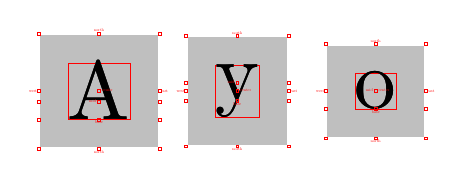
\begin{tikzpicture}
    \tikzstyle{ap}=[draw,rectangle,inner sep=0,red,very thin]
    \tikzstyle{apl}=[scale=0.15,red]
    \newcommand{\textnode}[2]{
        \path (#1,0) node[anchor=center,scale=3,fill=lightgray] (letter) {#2};
        \path (#1,0) node[anchor=center,scale=3,draw=red,ultra thin,inner sep=0] {#2};
        \path (letter.north) node[ap] {};
        \path (letter.north) node[anchor=south,apl] {north};
        \path (letter.north east) node[ap] {};
        \path (letter.north west) node[ap] {};
        \path (letter.center) node[ap] {};
        \path (letter.center) node[anchor=mid west,apl] {~center};
        \path (letter.east) node[ap] {};
        \path (letter.east) node[anchor=west,apl] {east};
        \path (letter.west) node[ap] {};
        \path (letter.west) node[anchor=east,apl] {west};
        \path (letter.mid) node[ap] {};
        \path (letter.mid) node[anchor=mid east,apl] {mid~~};
        \path (letter.mid east) node[ap] {};
        \path (letter.mid west) node[ap] {};
        \path (letter.base) node[ap] {};
        \path (letter.base) node[anchor=north,apl] {base};
        \path (letter.base east) node[ap] {};
        \path (letter.base west) node[ap] {};
        \path (letter.south) node[ap] {};
        \path (letter.south) node[anchor=north,apl] {north};
        \path (letter.south east) node[ap] {};
        \path (letter.south west) node[ap] {};
    }
    \textnode{0}{A}
    \textnode{5em}{y}
    \textnode{10em}{o}
\end{tikzpicture}

\begin{normalsize}
The only typographically meaningful anchors are ‘base’ and ‘mid’, and their ‘east’ and ‘west’ variants.
\par
\end{normalsize}


\end{document}
